\documentclass[10 pt]{article}

\usepackage[utf8x]{inputenc}
\usepackage{dsfont}
\usepackage{amsthm}
\usepackage{amsfonts}
\usepackage{amssymb}
\usepackage{tensor}
\usepackage{mathtools}
\usepackage[T1]{fontenc}
%\usepackage[spanish]{babel}
\usepackage[cm]{fullpage}
\usepackage{graphicx}
\usepackage{float}
\usepackage{bm}
\usepackage{setspace}
\usepackage{enumitem}
\usepackage{mdwlist}
\usepackage{parskip}
\usepackage{listings}
\usepackage{color}
%\usepackage{epstopdf}
\usepackage{tikz,datatool}
\usepackage{hyperref}

\newcommand{\HRule}{\rule{\linewidth}{0.5mm}}

\AtBeginDocument{
  \let\myThePage\thepage
  \renewcommand{\thepage}{\oldstylenums{\myThePage}}
}

\newcommand{\gra}{$^\text{o}$}
\newcommand{\dif}{\text{d}}
\newcommand{\avg}[1]{\left\langle #1 \right\rangle}
\newcommand{\ket}[1]{\left| #1 \right\rangle}
\newcommand{\bra}[1]{\left\langle #1 \right|}
\newcommand{\bket}[2]{\left\langle #1 \middle| #2 \right\rangle}
\newcommand{\der}[2]{\frac{\text{d} #1}{\text{d} #2}}
\newcommand{\prt}[2]{\frac{\partial #1}{\partial #2}}
\newcommand{\dert}[3]{\frac{\text{d}^#3 #1}{\text{d} #2^#3}}
\newcommand{\prtt}[3]{\frac{\partial^#3 #1}{\partial #2^#3}}
\newcommand{\dl}{\mathcal{L}}
\newcommand{\dha}{\mathcal{H}}
\newcommand{\vol}{\text{vol}}
\renewcommand{\vec}[1]{\pmb{#1}}

\newenvironment{algo}[1]
{  \begin{center}
   \mbox{
       \begin{minipage}{\textwidth}
           \begin{tabbing}
           \settabs
            #1
           \end{tabbing}
        \end{minipage}
    }
    \end{center}
}{}
\newcommand{\settabs}{mmm\=mmm\=mmm\=mmm\=mmm\=mmm\=\kill}

\DeclarePairedDelimiter\ceil{\lceil}{\rceil}
\DeclarePairedDelimiter\floor{\lfloor}{\rfloor}

\definecolor{mygray}{rgb}{0.4,0.4,0.4}
\definecolor{mygreen}{rgb}{0,0.5,0.25}
\definecolor{myorange}{rgb}{1.0,0.4,0}

\definecolor{clock0}{cmyk}{1,0,0,0}
\definecolor{clock1}{cmyk}{1,1,0,0}
\definecolor{clock2}{cmyk}{0,1,0,0}
\definecolor{clock3}{cmyk}{0,1,1,0}
\definecolor{clock4}{cmyk}{1,0,1,0}
\definecolor{clock5}{cmyk}{1,1,1,0}
\definecolor{clock6}{cmyk}{0,0,1,0}
\definecolor{clock7}{cmyk}{0,0,0,0.1}

\begin{document}

\lstset{
language=C++,
basicstyle=\ttfamily\color{black},
commentstyle=\color{mygray}\ttfamily,
frame=single,
numbers=left,
numbersep=5pt,
numberstyle=\tiny\color{mygray}\ttfamily,
keywordstyle=\color{mygreen}\ttfamily,
showspaces=false,
showstringspaces=false,
stringstyle=\color{myorange}\ttfamily,
tabsize=2,
emph={double,uint8_t,uint16_t,uint32_t,uint64_t,int8_t,int16_t,int32_t,int64_t},
emphstyle={\color{blue}\ttfamily}
}

\begin{center}
  \Large \textsc{Exercise 7: Grand-canonical Monte Carlo simulations near the critical point}
\end{center}

\begin{center}
  \large \textsc{Francisco García Flórez}
\end{center}

\section{Results}

\subsection{Dependence with $\mu^*$}

In the following plots we can see a histogram showing how many times the system has been found with an specific number of particles, what we will call $h(N)$. Since the number of particles is not an intensive property, instead of showing $N$ directly, we will divide by the volume in reduced units to find the density, which is indeed an intensive property.

\begin{figure}[H]
  \begin{center}
    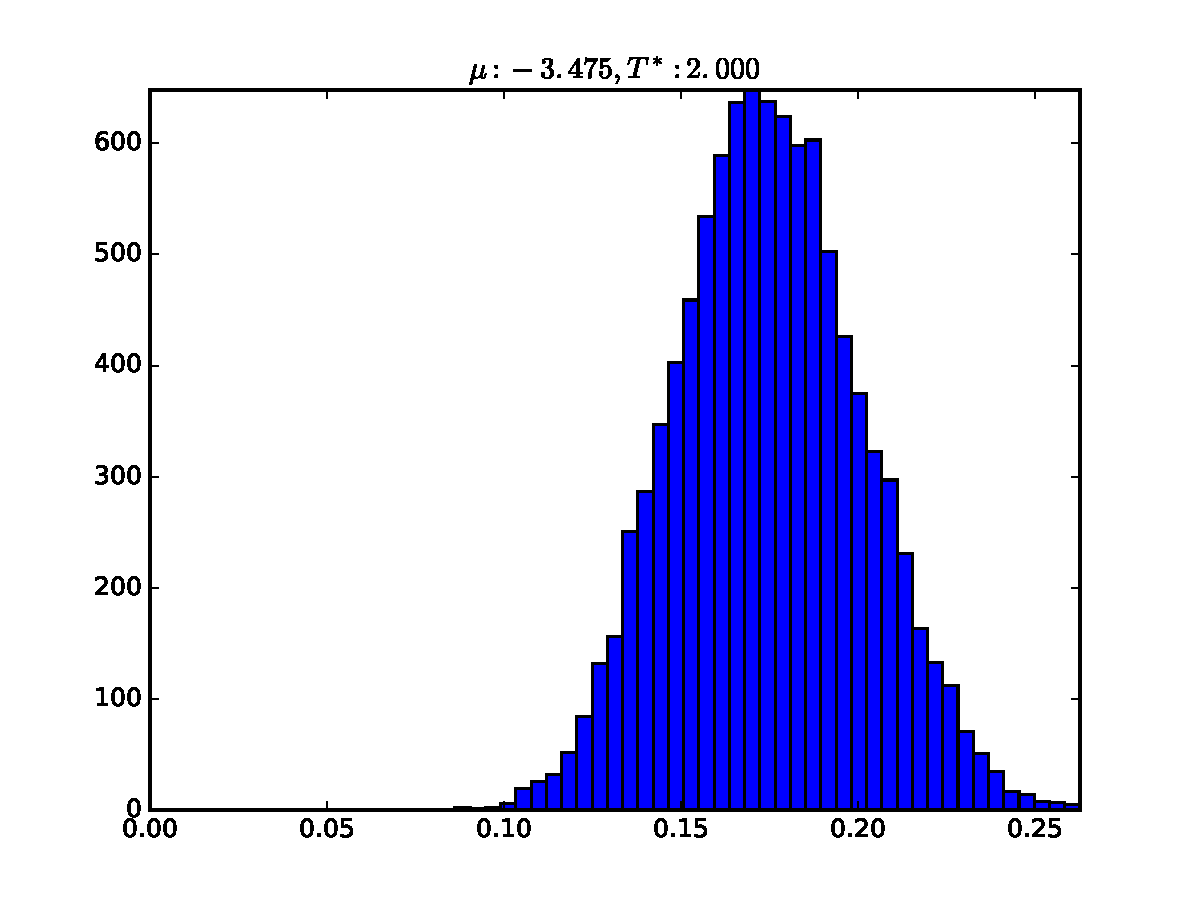
\includegraphics[width=0.49\textwidth]{{../graphs/hists-state/hist_-3.47500_2.00000}.pdf}
    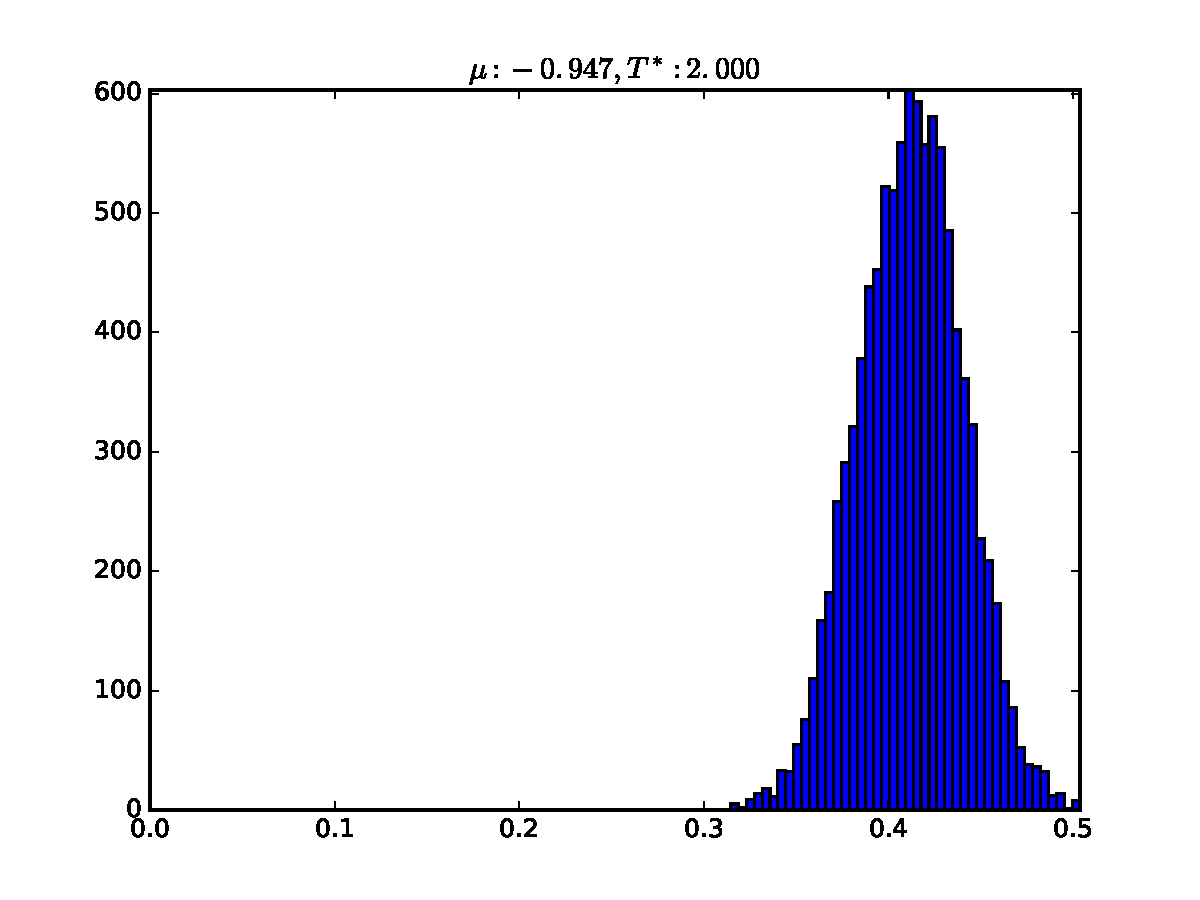
\includegraphics[width=0.49\textwidth]{{../graphs/hists-state/hist_-0.94737_2.00000}.pdf}
  \end{center}
  \begin{center}
    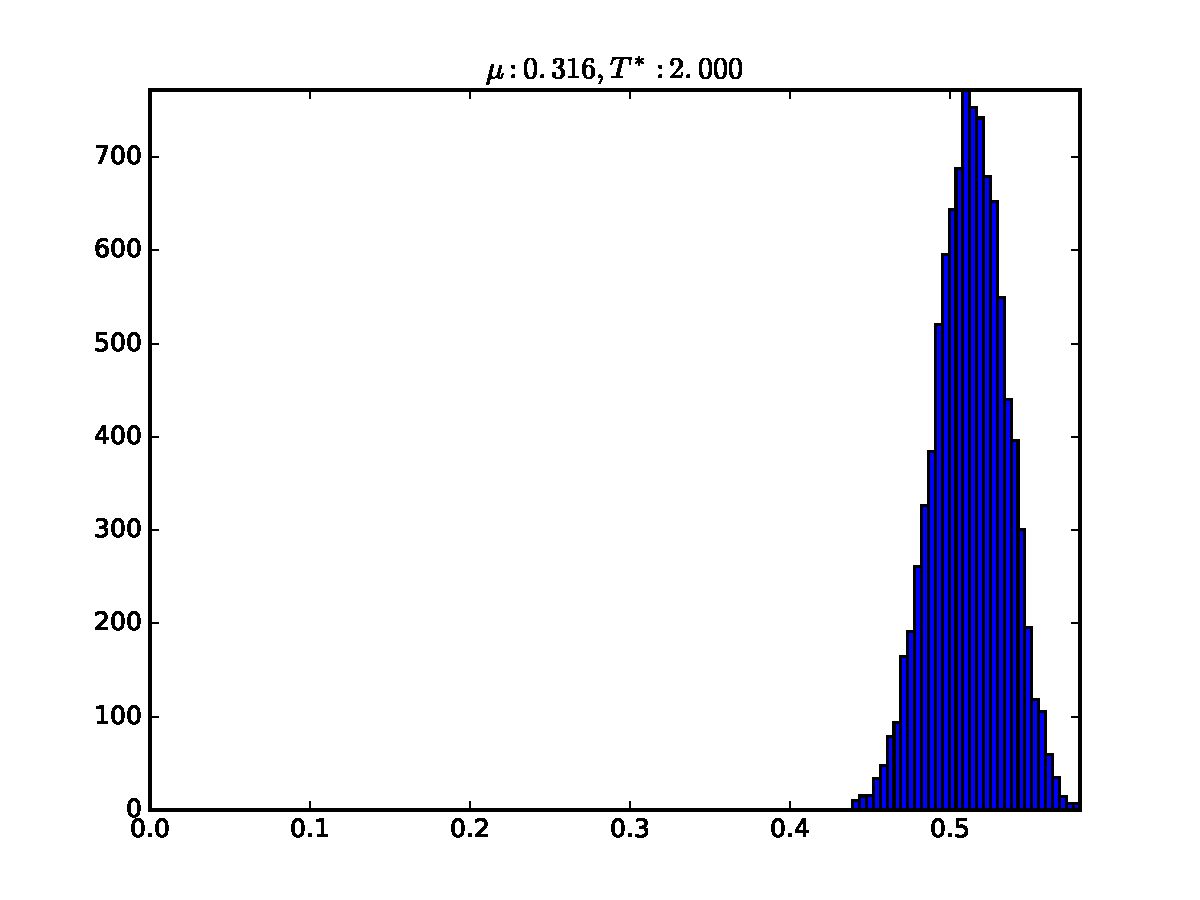
\includegraphics[width=0.49\textwidth]{{../graphs/hists-state/hist_0.31579_2.00000}.pdf}
    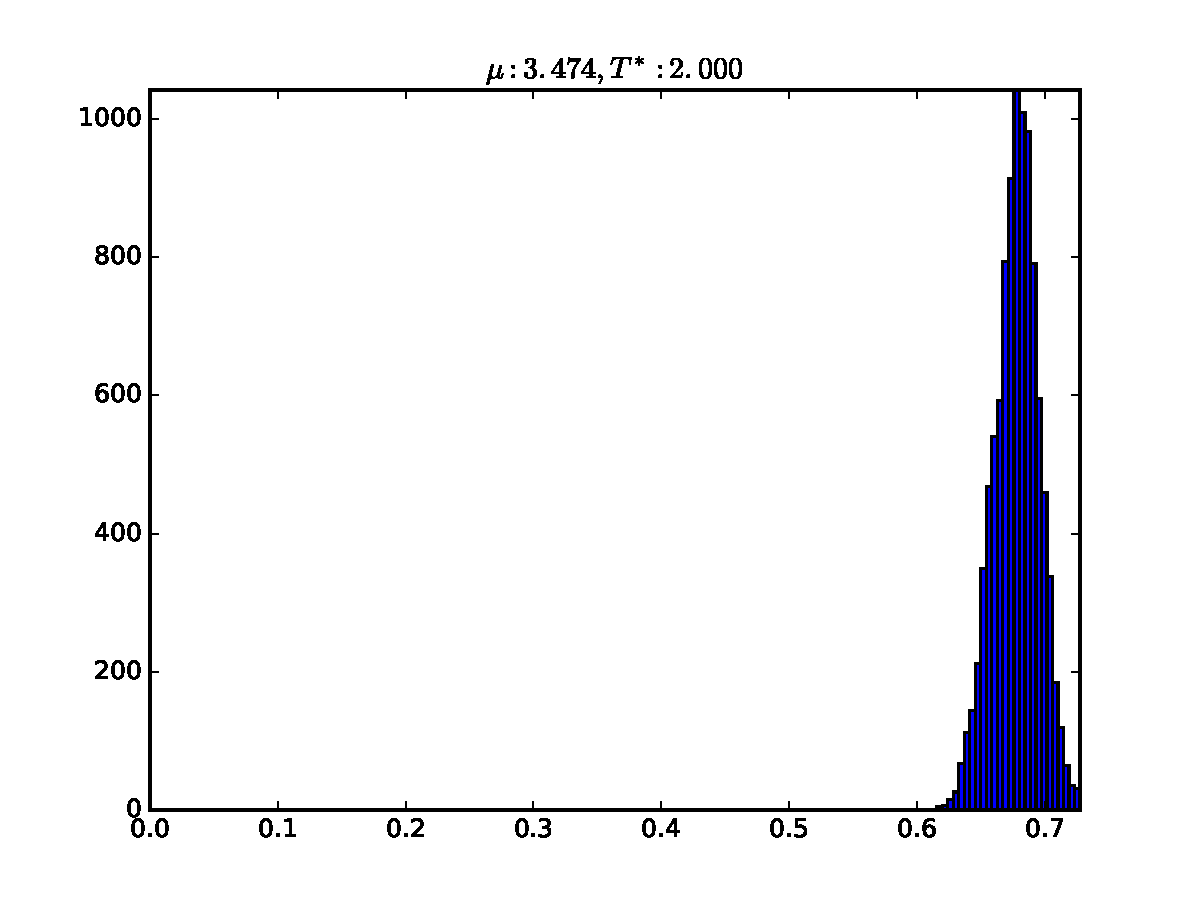
\includegraphics[width=0.49\textwidth]{{../graphs/hists-state/hist_3.47368_2.00000}.pdf}
  \end{center}
  \caption{Several histograms $h(\rho)$ for different values of $\mu$.}
\end{figure}

As expected, for lower values of $\mu^*$ the average density decreases, and increases for higher values. In the next section we will see a visual representation of this by looking at the equation of state $\mu - \rho$, and it will be clear how this value changes with $\mu$.

\subsection{Equation of state}

From simulations in the NVT ensemble we can expect certain values of $\mu$ as a function of the density, that we can compare in the following plot:

\begin{figure}[H]
  \begin{center}
    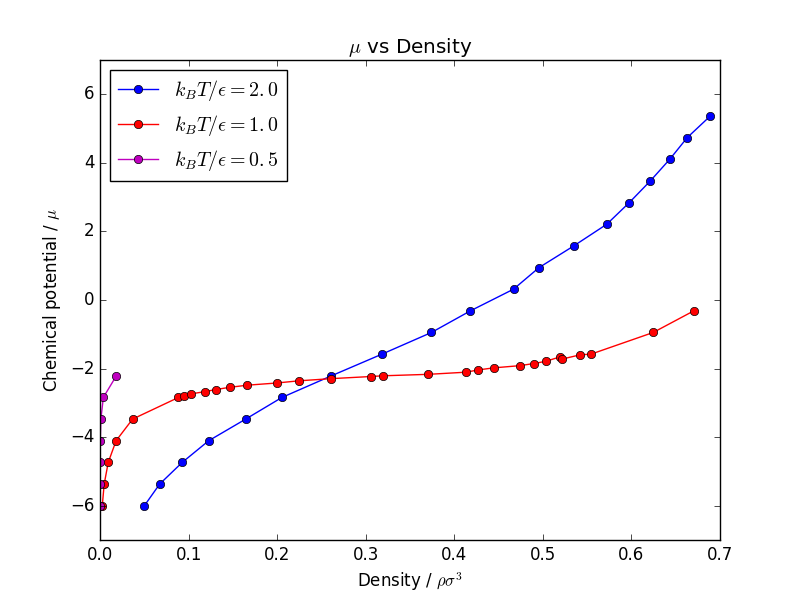
\includegraphics[width=0.7\textwidth]{{../graphs/mu_rho_low}.pdf}
  \end{center}
  \caption{Plot of the equation of state, where the dashed lines with triangles are the results from the NVT simulation.}
\end{figure}

As we can see, there is a remarkable agreement at low densities, and increasingly less for $\rho \sim 0.2$ and larger, possibly because we need either more steps in the simulation as the system has not equilibrated yet (in this case we have started from an initial configuration at low density) or we need more particles in the system.

Moreover, from this plot we can easily see the region where the critical point is located, so our search in the next section will be tightly bounded.

\subsection{Coexistence in the critical point}

As we can see in the following histograms, we have found several values of $(\mu^*, T^*)$ for which the system is in a liquid phase at the same time as a gas phase.

\begin{figure}[H]
  \begin{center}
    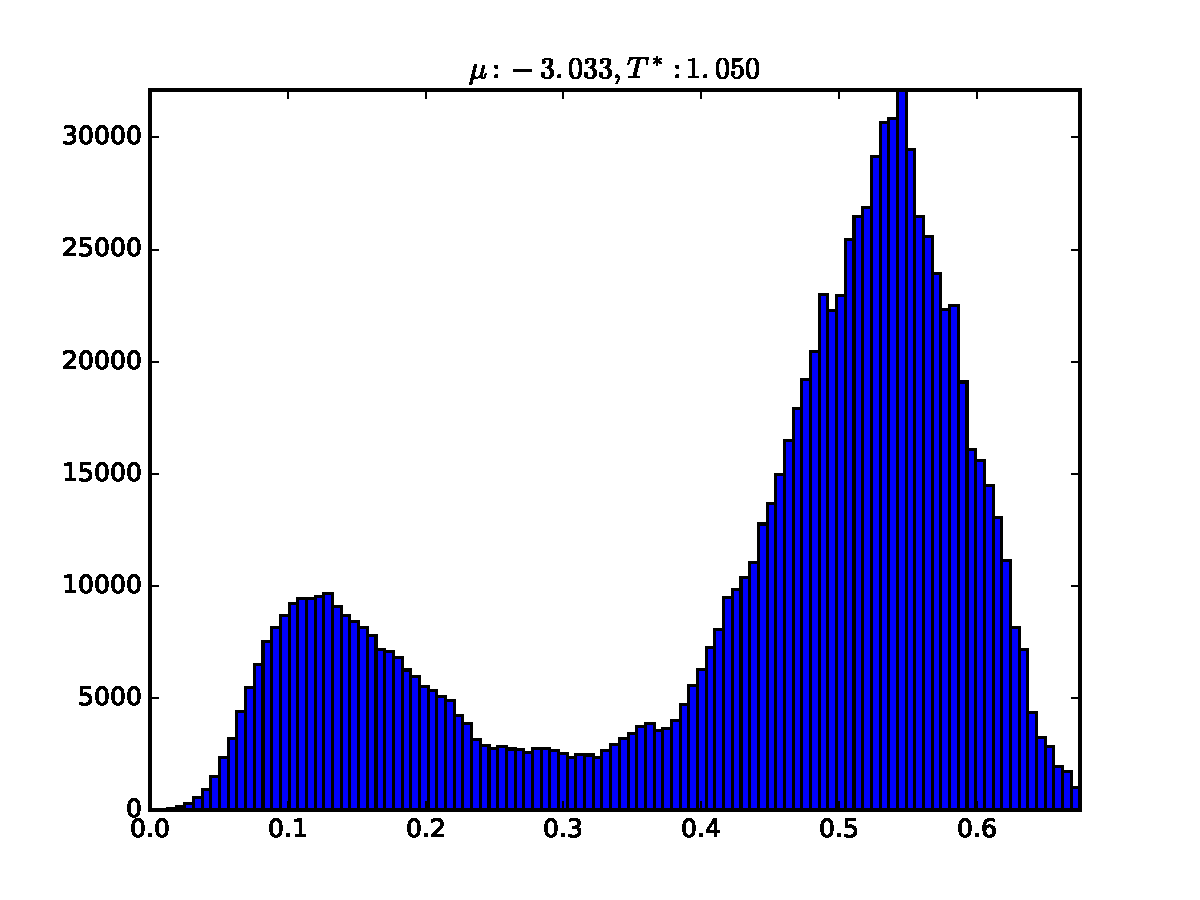
\includegraphics[width=0.49\textwidth]{{../graphs/hists/hist_-3.03333_1.05000}.pdf}
    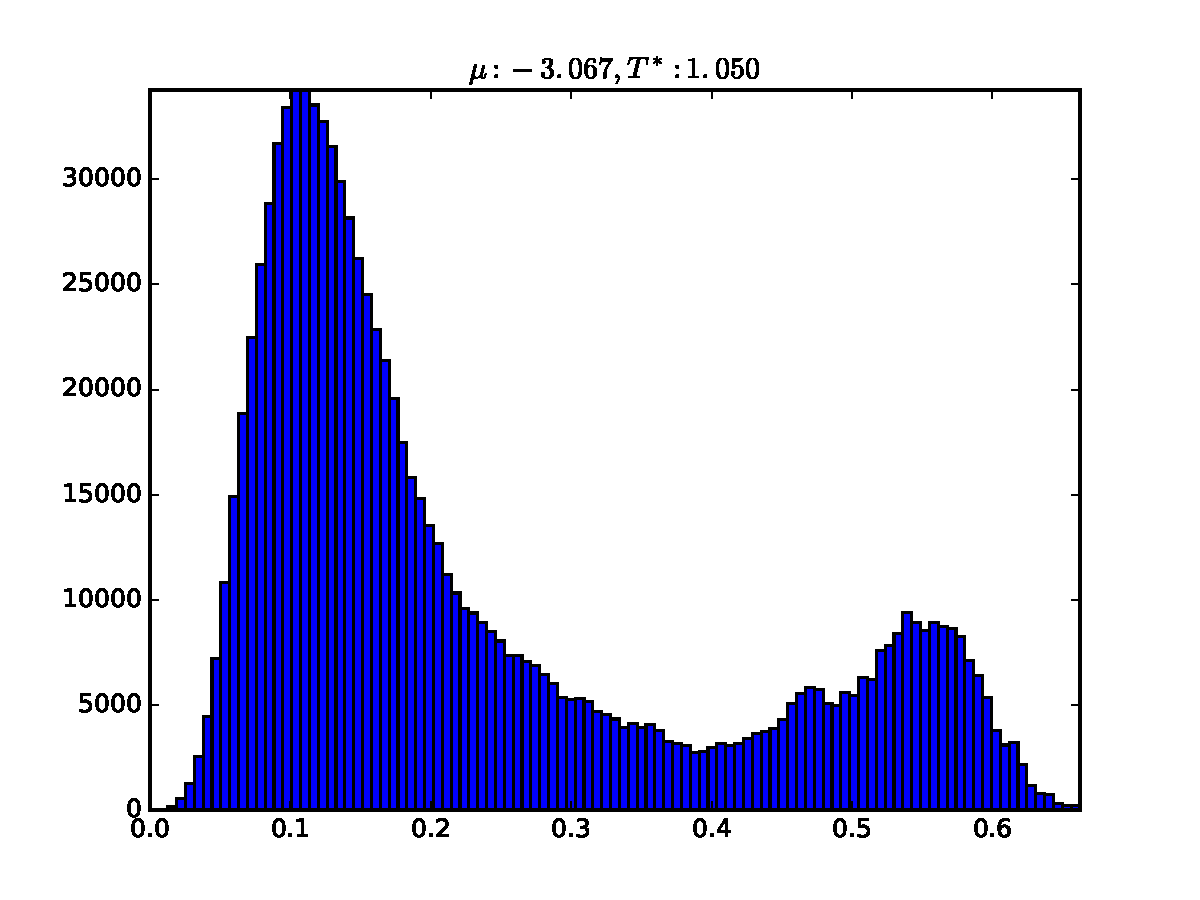
\includegraphics[width=0.49\textwidth]{{../graphs/hists/hist_-3.06667_1.05000}.pdf}
  \end{center}
  \begin{center}
    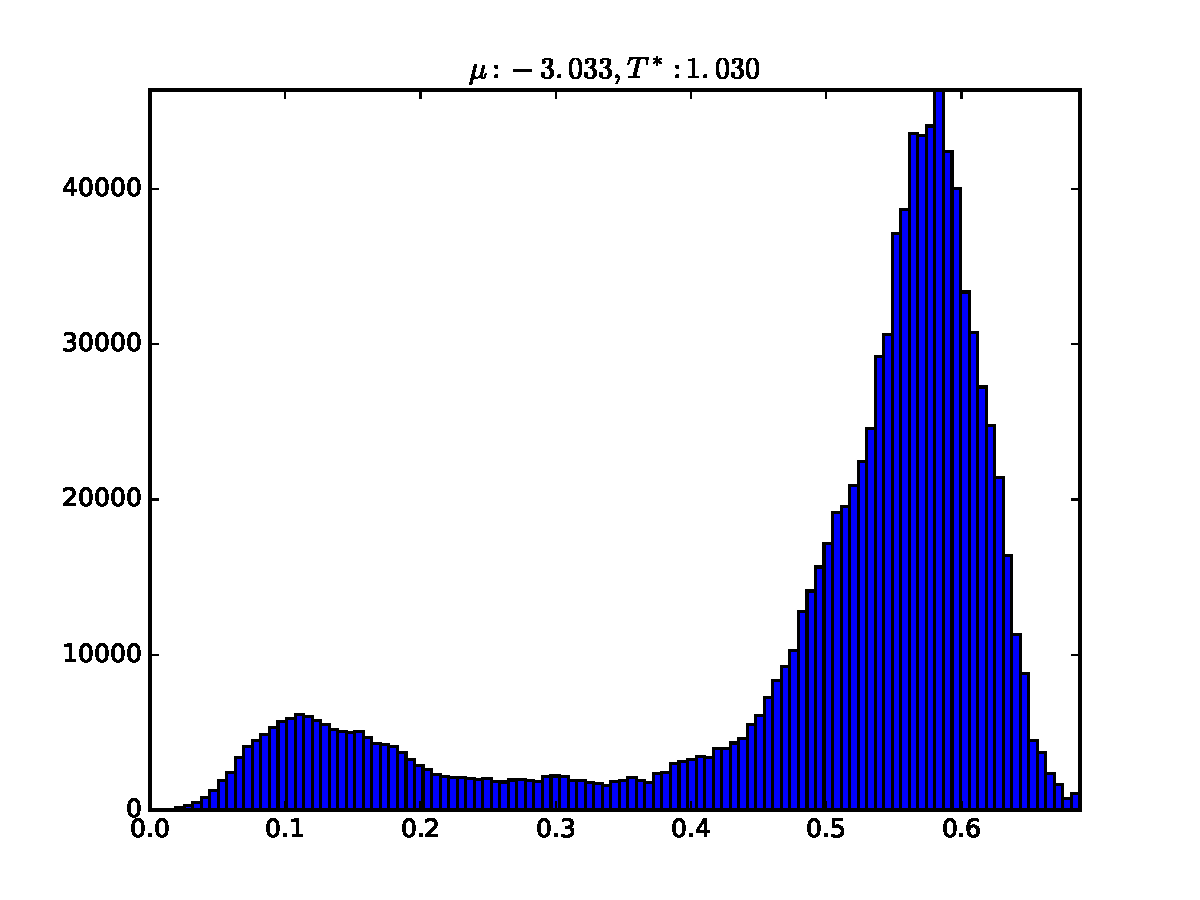
\includegraphics[width=0.49\textwidth]{{../graphs/hists/hist_-3.03333_1.03000}.pdf}
    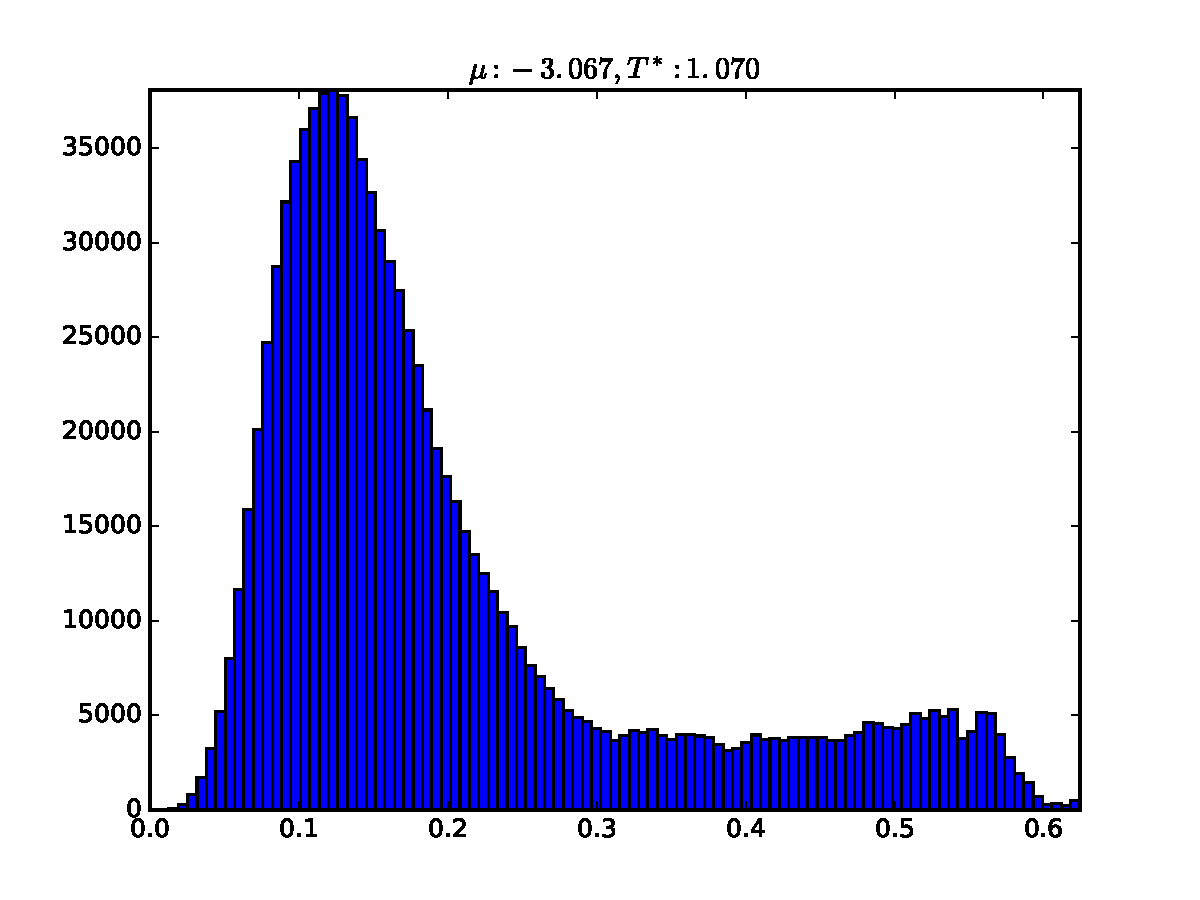
\includegraphics[width=0.49\textwidth]{{../graphs/hists/hist_-3.06667_1.07000}.pdf}
  \end{center}
  \caption{Several histograms $h(\rho)$ for different values of $\mu^*$ and $T^*$, showing coexistence.}
\end{figure}

By performing several simulations with different values of $\mu^*$ it is possible to find one for which the height of the peaks is approximately the same:

\begin{figure}[H]
  \begin{center}
    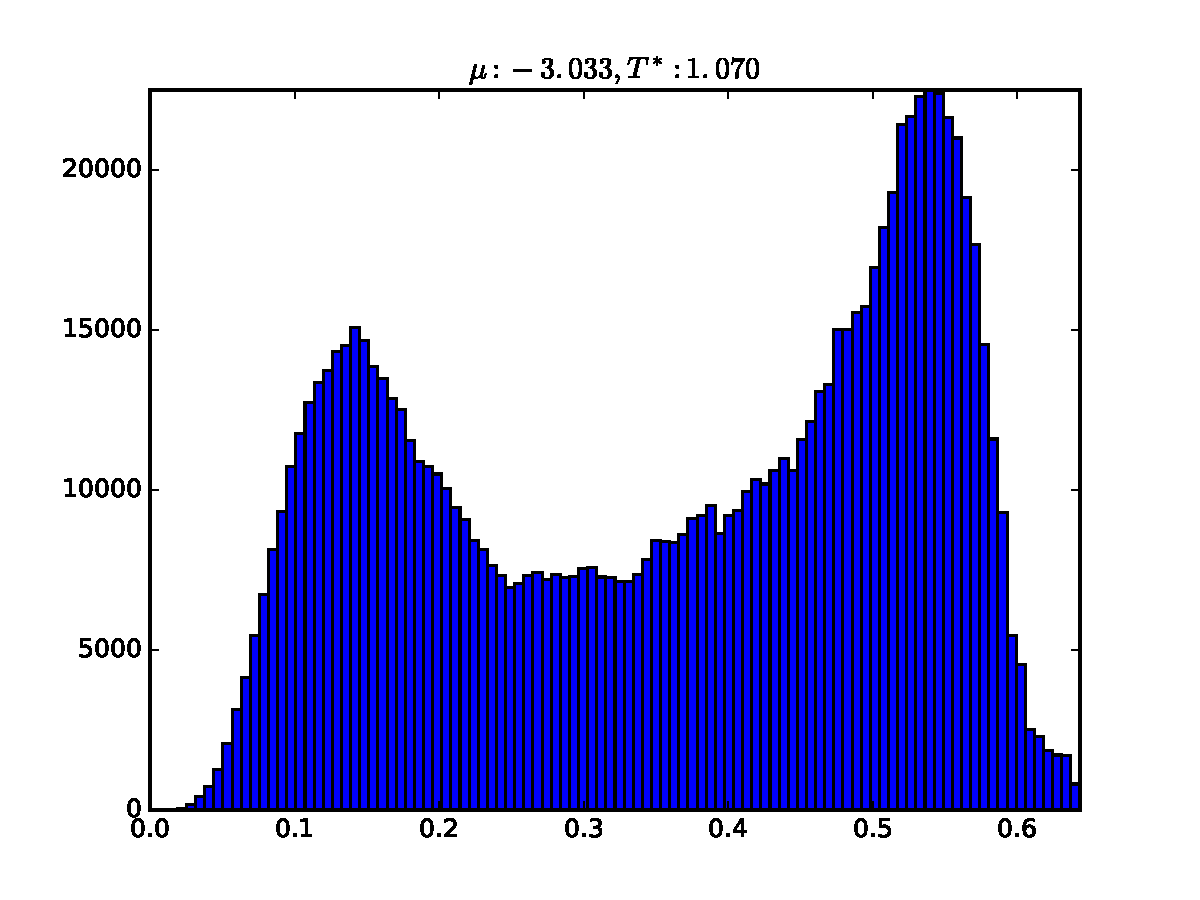
\includegraphics[width=0.49\textwidth]{{../graphs/hists/hist_-3.03333_1.07000}.pdf}
    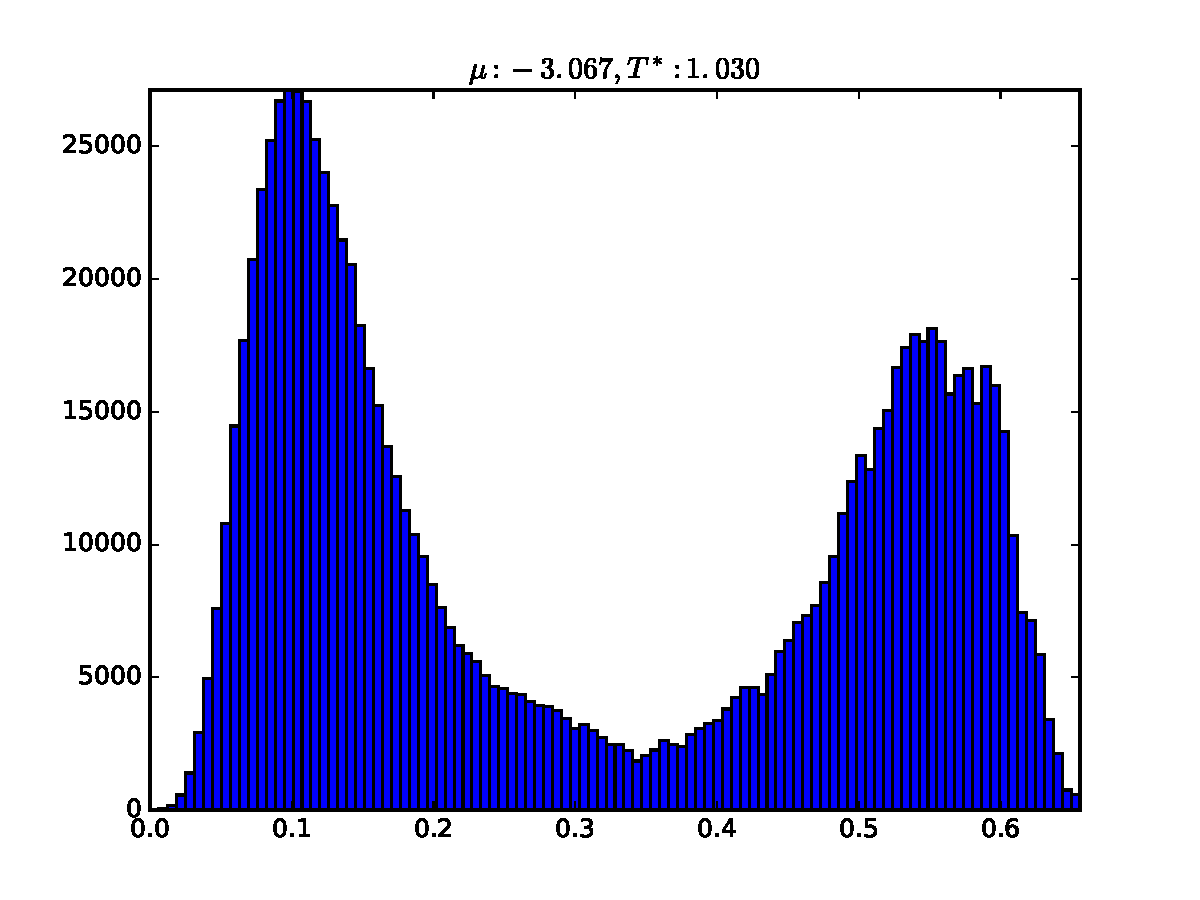
\includegraphics[width=0.49\textwidth]{{../graphs/hists/hist_-3.06667_1.03000}.pdf}
  \end{center}
  \caption{Histogram showing same-height peaks.}
\end{figure}

Plotting now these simulation's results in the $\rho - T^*$ plane we can see the following:

\begin{figure}[H]
  \begin{center}
    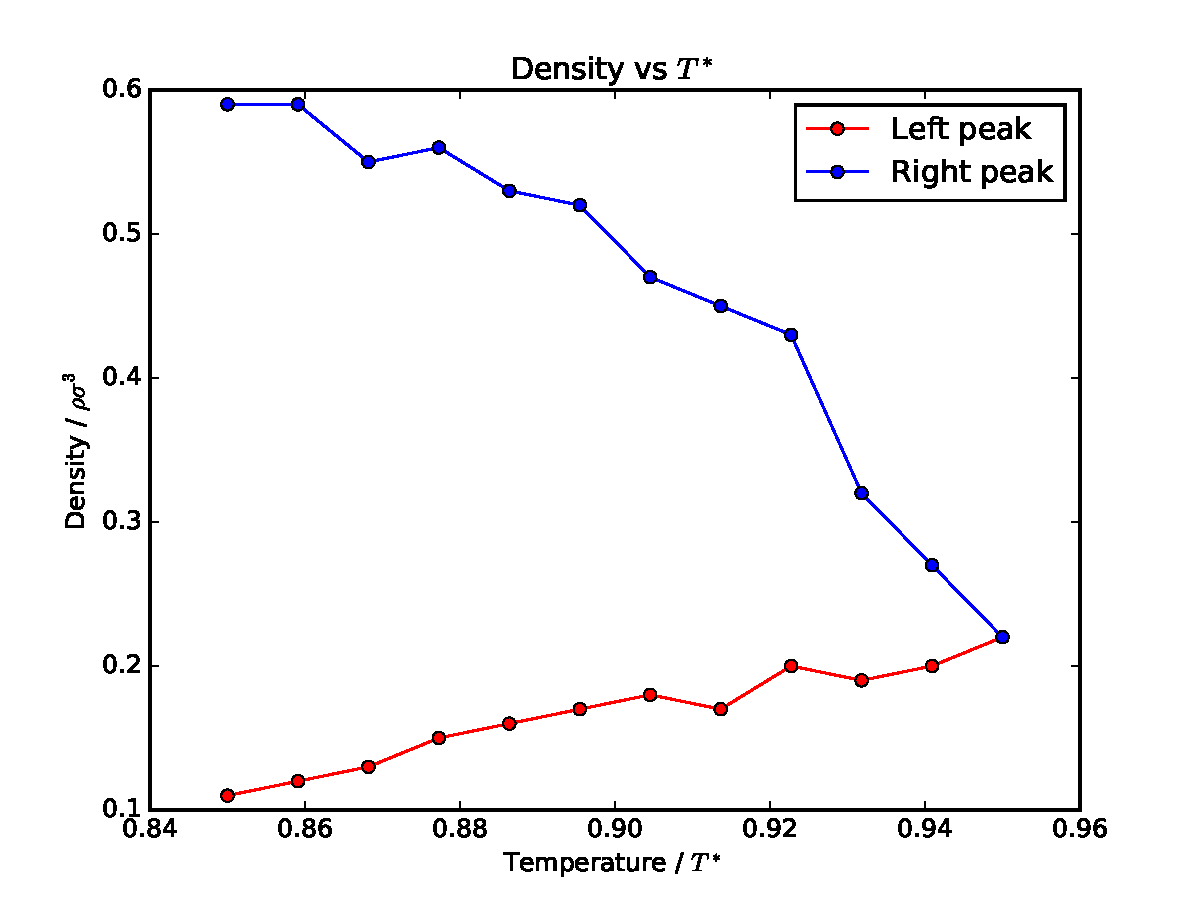
\includegraphics[width=0.7\textwidth]{{../graphs/d_peak_rho}.pdf}
  \end{center}
  \caption{Plot of the density of each phase as a function of temperature.}
\end{figure}

Here we can see a more-or-less linear relation for $\rho(T^*)$, which if we consider that the right peak is not completely resolved because we start with a low density configuration, a linear behavior is well inside the error bars. Although, we would expect to find a power-law relation instead. It's possible to explain the functional dependence we find for the left peak by looking at the box size we are using, because for smaller boxes the number of particles will not change a lot, and thus for low densities any significant change of the number of particles would be a significant portion of the system, therefore making difficult to see any significant change in this function.

On the other hand, for the right peak we don't have this limitation and thus the shape is closer to a power law as we were expecting. Even in this plot we are not representing any error bars, the method used to compute this values (by hand) introduces quite large amounts of error, so we can expect not to find a particularly good approximation of the functional dependence for the right peak. This can be improved by using a high density initial configuration and focus in the right peak, instead of starting from a low density configuration for both.

Finally, $h(N)$ can be physically interpreted as the distribution density function of the particle number in the system, and can be related to the free energy if we consider that this energy is related to the derivative of the chemical potential with respect to the number of particles.

On the other hand, this method is clearly not going to work for low densities, as $\beta$ in this case will be so high that any particle addition or subtraction will be unlikely to happen, and thus any simulation would take an unreasonable amount of time.

\subsection{Representation}

Finally we are going to visually compare two sets of snapshots of the system, simulated in the NVT ensemble with values of $\mu$, $T$ and $\rho$ such that it's in the middle of two peaks.

\begin{figure}[H]
  \begin{center}
    \includegraphics[width=0.49\textwidth]{{../graphs/coex}.pdf}
    \includegraphics[width=0.49\textwidth]{{../graphs/coex-close}.pdf}
  \end{center}
  \begin{center}
    \includegraphics[width=0.49\textwidth]{{../graphs/high}.pdf}
    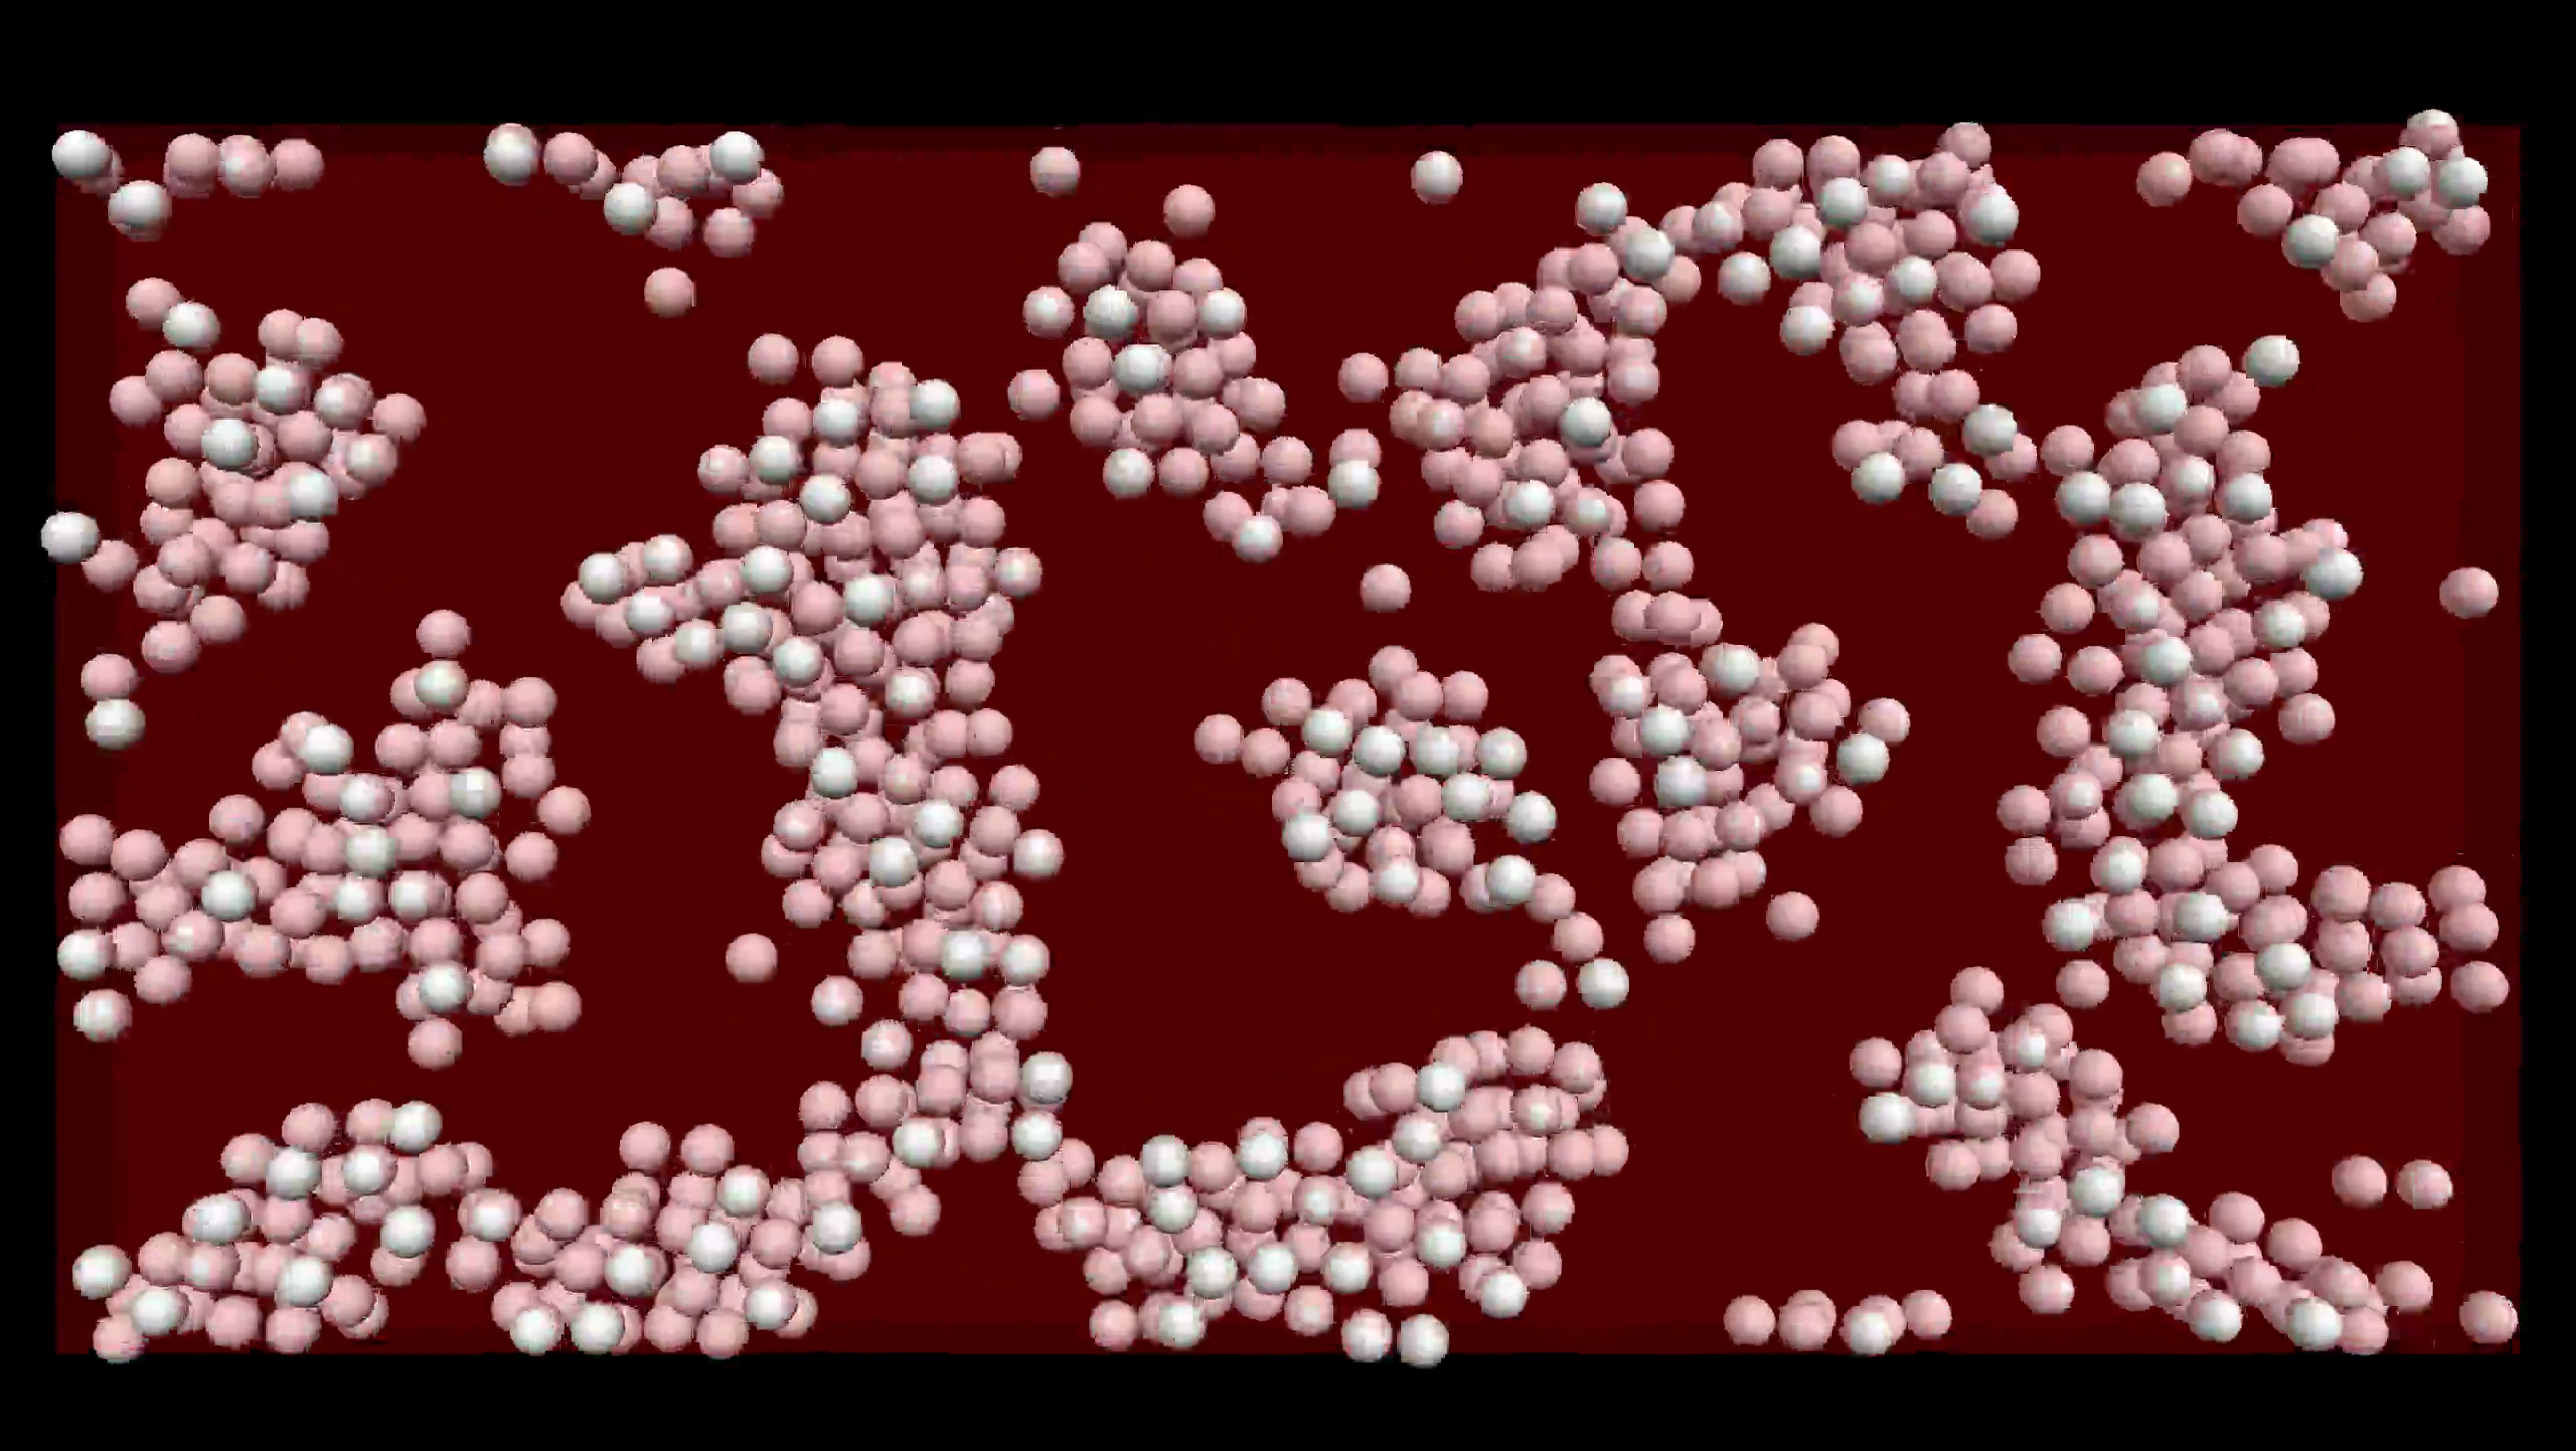
\includegraphics[width=0.49\textwidth]{{../graphs/low}.pdf}
  \end{center}
  \caption{Several snapshots of the system, in the critical point (top left) near the critical point (top right) and far away from it, for low $T^*$ (bottom right) and high $T^*$ (bottom left). A few movies can be seen at \url{https://www.youtube.com/playlist?list=PL96WXaDFF_IzW-FmyGbG4ad_L8_exNoBf}}
\end{figure}

We can notice that near the critical point there are regions with high density, in liquid phase, and others with way less particles, in the gas phase. On the other hand, when we get far away from it, the system clearly behaves again as a liquid, when decreasing $T^*$, or as a gas for high $T^*$.

Since the interfacial tension keeps particles together, when the system is close to the critical point it should increase, so particles in the liquid phase can be together.

\end{document}
